% This document is available under the Creative Commons Attribution-ShareAlike
% License; additional terms may apply. See
%   * http://creativecommons.org/licenses/by-sa/3.0/
%   * http://creativecommons.org/licenses/by-sa/3.0/legalcode
%
% Copyright 2010 Jérôme Pouiller <jezz@sysmic.org>
%

\part{Modules noyau}

{
\setbeamertemplate{background canvas}{}
\begin{frame}[plain]
  \partpage
  \begin{textblock}{10}(6,11)
    %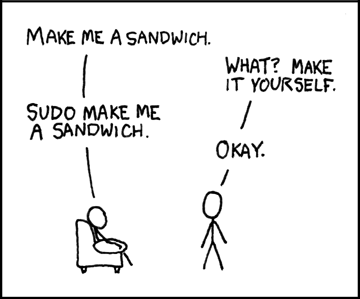
\includegraphics[height=30mm,width=30mm]{sandwich}
    \begin{quote}
      \rmfamily\textit\textbf\color{darkgray}{\large
        ``Q: How many programmers does it take to change a light bulb?\\
        A: None -- It’s a hardware problem.''}
      %\vskip3mm\hspace*\fill{\small--- William Shakespeare, Hamlet}
    \end{quote}
  \end{textblock}
\end{frame}
}

\begin{frame}
  \tableofcontents
\end{frame}


%\section{Options principales du noyau}
%
%\subsection{Configuration globale}
%
%\begin{frame}[fragile=singleslide]{Configuration globale}
%  \emph{General setup}:
%  \begin{itemize} 
%  \item \emph{Prompt for  development and/or incomplete code/drivers}:
%    Débloque  les  options  de  compilation  pour  les  drivers/option
%    instables (staging, etc...)
%  \item  \emph{Cross-compiler  tool  prefix}  :  Affecte  la  variable
%    \c{CROSS_COMPILE}
%  \item   \emph{Local  version}   :   Ajoute  un   identifiant  à   la
%    version. Indispensable  dans les phases  d'intégration. La version
%    peut être lue dans  \file{/proc/version}. Il est aussi possible de
%    faire \c{make kernelrelease} dans  un répertoire de compilation du
%    noyau.
%  \item  \emph{Automatically  append  version  information}  :  Ajoute
%    l'identifiant git  à la version. Indispensable dans  les phases de
%    développement
%  \item \emph{Kernel  compression mode}: Permet de choisir  le type de
%    compression.   Chaque  algorithme   a  ces  inconvénients  et  ses
%    intérêts.
%    \note[item]{cf. \url{http://free-electrons.com/blog/lzo-kernel-compression}}
%  \item \c{SWAP}: Permet de gérer un espace d'échange dur un disque
%  \end{itemize}
%\end{frame}
%
%\begin{frame}[fragile=singleslide]{Configuration globale}
%  \begin{itemize} 
%  \item  \c{SYSVIPC} et  \c{MQUEUE}:  Communication inter-processus
%    définis par Posix
%  \item \c{IKCONFIG}: Embarque le \file{.config} dans le noyau 
%  \item  \c{EXPERT} et  \c{EMBEDDED} Débloque  les  options permettant
%    principalement  de réduire la  taille du  noyau en  supprimant des
%    modules importants
%  \item \c{CC_OPTIMIZE_FOR_SIZE}: Compile avec \c{-Os}
%  \item \c{KPROBES},  \c{PERF_EVENTS}, \c{PROFILING}, \c{GCOV_KERNEL}:
%    Active les différentes instrumentations du noyau
%  \end{itemize} 
%\end{frame}
%
%\begin{frame}[fragile=singleslide]{Les périphériques de block}
%  \c{MODULES}: Active la gestion des modules
%  \\[2ex]
%  \c{BLOCK}: Il est possible  de désactiver la gestion des périphérique
%  de block si votre système n'utilise que de la mémoire flash.
%  \begin{itemize} 
%  \item \emph{IO  Schedulers}: Permet de choisir  un ordonnanceur d'E/S
%    différent de celui proposé en standard
%  \end{itemize} 
%  \emph{System type}:
%  \begin{itemize} 
%  \item Permet de choisir le type d'architecture et de chipset
%  \item Il est  possible de désactiver certains cache  lors des phases
%    de développement
%  \item Vous trouverez aussi dans  ce menu les options relative au jeu
%    d'instructions accepté
%  \end{itemize}
%\end{frame}
%
%\subsection{Fonctionnalités du noyau}
%
%\begin{frame}[fragile=singleslide]{Options de l'horloges}
%  \emph{Kernel features}
%  \begin{itemize} 
%  \item \c{HZ} (pas sur ARM): Définit l'intervalle de réordonnancement
%    de l'ordonnanceur.   Plus cette valeur est  forte, plus l'overhead
%    introduit par le changement de  contexte est important et plus les
%    temps de réponses des tâches sont courts
%  \item \c{NO_HZ}: Permet de rendre la période de réordonnancement des
%    tâches  dynamique.   Devrait  permettre  un  léger   gain  de  CPU
%    (finalement  négligeable avec  l'ordonnanceur  en $o(1)$).  Permet
%    surtout de gagner en consommation électrique.
%  \item   \c{HIGH_RES_TIMER}:  Gère  les   timers  avec   une  horloge
%    différente de  l'ordonnanceur (l'horloge  est alors géré  comme un
%    périphérique  à  part).    Permet  d'obtenir  une  bien  meilleure
%    précision sur les mesure de  temps, à condition que votre matériel
%    possède une horloge \emph{HighRes}.
%  \end{itemize}
%\end{frame}  
%
%\begin{frame}[fragile=singleslide]{Options de l'ordonnanceur}
%  \begin{itemize} 
%  \item  \emph{Preemption Model}:  Permet d'activer  la  préemption du
%    noyau. Le pire  temps réponse sont améliorés, mais  le temps moyen
%    est généralement  moins bon.  Un noyau  préemptif stresse beaucoup
%    plus  de  code.  Ne  pas  activer  si  vous utilisez  des  drivers
%    extérieur non garanti pour cette option.
%  \item \c{RT_PREEMPT} (sur certaines architectures seulement): Permet
%    de threader  les IRQ  et ainsi de  remplacer les spinlock  par des
%    mutex.  Ajoute un protocole  d'héritage de priorité aux mutex.  Le
%    kernel devient alors totalement  préemptif.  A n'utilisez que lors
%    d'application  temps   réelle.   Etudiez  des   solutions  à  base
%    d'hyperviseurs.
%  \item Ne confondez pas la préemption du noyau avec la préemption des
%    tâches utilisateur.
%  \end{itemize}
%\end{frame}  
%
%\begin{frame}[fragile=singleslide]{Option de gestion de la mémoire}
%  \begin{itemize} 
%  \item \c{EABI},  \c{OABI}, etc...  : Différentes format  d'appel des
%    fonctions. Spécifique à ARM (mais très important)
%  \item  \emph{Memory Model}: Permet  de gérer  les futurs  systèmes à
%    mémoire asymétriques entre les CPU
%  \item  \c{COMPACTION}:  Permet de  compresser  les  page de  mémoire
%    plutôt  que les mettre  en swap.  Particulièrement utile  dans les
%    systèmes sans swap !
%  \item  \c{KSM}: Permet  de  fusionner les  page mémoire  identiques.
%    Uniquement   utile   avec   des   machines   virtuelles   ou   des
%    chroot. Sinon, les  noyau sait que le fichier  est déjà en mémoire
%    et ne duplique pas la page
%  \end{itemize} 
%\end{frame}
%
%\subsection{Les options de boot}
%
%\begin{frame}[fragile=singleslide]{Configuration du boot et du FPE}
%  \emph{Boot options}:
%  \begin{itemize}
%  \item \emph{Flattened Device  Tree} : Utilise \emph{OpenFirmware}, le
%    nouveau format de  description matériel appelé aussi \emph{Flatten
%      Device Tree}
%  \item  \emph{Default kernel  command string}:  Permet de  passer des
%    paramètres  par défaut  au noyau  (nous verrons  cela un  peu plus
%    loin)
%  \item \emph{boot loader address}:  Permettent de démarrer le noyau à
%    partir d'une ROM, d'une MMC, etc...
%  \item \emph{Kernel Execute-In-Place  from ROM}: Permet d'exécuter un
%    noyau non compressé à partir d'une ROM
%  \end{itemize}
%  \emph{Floating point emulation}: Si  une instruction sur des nombres
%  à virgule flottante est rencontrée  et ne peut pas être exécutée, le
%  noyau peut alors émuler l'instruction (voir aussi \c{-msoft-float})
%\end{frame}
%
%\subsection{Le réseau}
%
%\begin{frame}[fragile=singleslide]{Configuration réseau}
%  \emph{Networking}:
%  \begin{itemize}
%  \item Possibilité  d'activer les innombrables  protocoles réseaux de
%    niveaux 1, 2 et 3
%  \item  \emph{Network options} : Beaucoup  de fonctionnalité  réseau :
%    client dhcp,  bootp, rarp, ipv6, ipsec, les  protocole de routage,
%    gestion de QoS, support des VLAN, du multicast,
%  \item   \emph{Unix  domain  sockets}   :  Les   sockets  \emph{UNIX}
%    (cf. sortie de \c{netstat})
%  \item   \emph{TCP/IP   networking}  :   Les   sockets  bien   connue
%    \emph{TCP/IP}
%  \item  \emph{Netfilter}  :  Le  firewall  de  Linux.   D'innombrable
%    options.  Permet l'utilisation d'iptables si l'option \c{IPTABLES}
%    est active.
%  \end{itemize} 
%\end{frame}
%
%\subsection{Les systèmes de fichiers}
%
%\begin{frame}[fragile=singleslide]{Configuration des systèmes de fichiers}
%  \emph{File systems}:
%  \begin{itemize}
%  \item   \emph{Second   extended},   \emph{Ext3  journalling   file},
%    \emph{The Extended 4 filesystem}: Le file system standard de Linux
%  \item \emph{FUSE}: Permet de  développer des systèmes de fichiers en
%    espace utilisateur
%  \item \emph{Pseudo  filesystems} Systèmes de  fichiers sans supports
%    physiques
%    \begin{itemize} 
%    \item \c{TMPFS}: File system  volatile en RAM.  Très utilisé avec
%      des système en flash vu que  l'accès à la Flash est coûteux en
%      temps et destructeur pour la flash
%    \item \c{SYSFS} et \c{PROC_FS}:  Permettent au noyau d'exporter un
%      certain  nombre de  donnée interne  vers le  userland.  Beaucoup
%      d'outils  système tirent  lors informations  de ces  systèmes de
%      fichiers.  Ils  doivent être montés dans  \c{/sys} et \c{/proc}.
%      \c{/proc} est  plutôt orienté  processus alors que  \c{/sys} est
%      orienté modules et paramétrage du noyau.
%    \end{itemize} 
%  \end{itemize}
%\end{frame}
%
%\begin{frame}[fragile=singleslide]{Configuration des systèmes de fichiers}
%  \begin{itemize}
%  \item  \emph{Miscellaneous  filesystems}  Contient des  systèmes  de
%    fichiers spécifiques
%    \begin{itemize} 
%    \item  \emph{eCrypt filesystem layer}  : Gestion  transparent d'un
%      file system codé
%    \item \emph{Journalling  Flash File  System v2} :  Spécialisé pour
%      les  Flash avec  gestion de  l'écriture uniforme,  des \emph{bad
%        blocks} et des \emph{erase blocks}.
%    \item \emph{Compressed ROM file  system}: Spécialisé pour ROM sans
%      accès en écriture.
%    \item  \emph{Squashed   file  system}:  Idem   \emph{cramfs}  mais
%      fortement compressé
%    \end{itemize} 
%  \item \emph{Network File Systems}
%    \begin{itemize}
%    \item \emph{NFS client support}  : File system sur ethernet.  Très
%      utilisé dans l'embarqué durant les phases de développement
%    \item \emph{Root file system on  NFS}: Permet de démarrer le noyau
%      sur une partition NFS
%    \end{itemize} 
%  \end{itemize} 
%\end{frame}
%
%\subsection{Les drivers}
%
%\begin{frame}[fragile=singleslide]{Configuration des Drivers}
%  \emph{Device Drivers} Des centaines de drivers. Notons:
%  \begin{itemize}
%  \item   \emph{path to uevent helper}:  Le  programme   apellé  lorsqu'un
%    nouveau            périphérique            est           détecté
%    (cf.              \c{/proc/sys/kernel/hotplug}             et
%    \c{/sys/kernel/uevent_helper})
%  \item  \emph{Maintain a devtmpfs  filesystem to  mount at  /dev}: Un
%    tmpfs  spécifique  pour  les  devices  automatiquement  monté  sur
%    \file{/dev}.   Les  fichiers  devices sont  alors  automatiquement
%    créés sans l'aide d'un programme extérieur.
%  \item \emph{Memory Technology Device}: Les flashs
%  \item \emph{Staging drivers}: Des drivers en cours de bêta
%  \end{itemize} 
%\end{frame}
%
%\subsection{Autres options}
%
%\begin{frame}[fragile=singleslide]{Configuration du noyau}
%  Mais aussi:
%  \begin{itemize} 
%  \item \emph{Kernel  Hacking}:  Options  concernant le  débugging  du
%    noyau. % Nous y reviendrons dans la section Debug
%  \item  \emph{Security  Options}:  Plusieurs framework  permettant  de
%    gérer des  droits plus  fin sur les  programmes exécutés  et/ou de
%    garantir l'intégrité des donnée à l'aide de TPM.
%  \item   \emph{Cryptographic   API}:   Fonctions   de   cryptographies
%    sélectionnées     automatiquement     par     d'autres     modules
%    (particulièrement les protocoles réseaux)
%  \item  \emph{Library routines}: Idem  \emph{Cryptographic API}  mais
%    avec principalement des calculs de checksum.
%  \end{itemize} 
%\end{frame}
%
\section{Création de modules}

\subsection{Template}

\begin{frame}[fragile=singleslide]{Les modules noyau}{my\_module}
  \lstinputlisting[language=c,firstline=16]{samples/mod0_min/mod0_min.c}
\end{frame}

\begin{frame}[fragile=singleslide]{Quelques macros de base}
  Ces macros  permettent de placer  des informations sur  des symboles
  particulier dans module;
  \begin{itemize} 
  \item Déclare la fonction à apeller lors du chargement du module
    \begin{lstlisting} 
module_init
    \end{lstlisting} 
  \item Déclare la fonction à appeller lors du déchargement du modules
    \begin{lstlisting} 
module_exit
    \end{lstlisting} 
  \item Déclare un paramètre
    \begin{lstlisting}
module_param
    \end{lstlisting}
  \item Documente un paramètre pour modinfo
    \begin{lstlisting}
MODULE_PARM_DESC
    \end{lstlisting}
  \item Déclare un auteur du fichier. Peut apparaitre plusieurs fois.
    \begin{lstlisting}
MODULE_AUTHOR
    \end{lstlisting}
  \end{itemize}
\end{frame}
\begin{frame}[fragile=singleslide]{Quelques macros de base}
  \begin{itemize} 
  \item Description du modules
    \begin{lstlisting}
MODULE_DESCRIPTION
    \end{lstlisting}
  \item License. Indispensable
    \begin{lstlisting}
MODULE_LICENSE
    \end{lstlisting}
  \item Version du module
    \begin{lstlisting}
MODULE_VERSION
    \end{lstlisting}
  \item Rend le symbole visible par les autres modules.  Il sera alors
    pris en compte dans le calcul des dépendances de symboles.
    \begin{lstlisting}
EXPORT_SYMBOL
    \end{lstlisting} 
  \item Idem \cmd{EXPORT\_SYMBOL} mais  ne permet sont utilisation que
    pour les modules GPL
    \begin{lstlisting}
EXPORT_SYMBOL_GPL
    \end{lstlisting} 
  \end{itemize}
\end{frame}

\subsection{Licences}

\begin{frame}[fragile=singleslide]{Parlons des licenses}
  Le noyau est sous license GPL. Néanmoins, le débat est ouvert sur la
  possibilité  qu'un module  propriétaire puisse  se linker  avec.  Le
  débat n'est pas  tranché. Le noyau laisse la  posisbilité à l'auteur
  d'exporter   ses   modules   avec   \verb+EXPORT_SYMBOL+   ou   avec
  \verb+EXPORT_SYMBOL_GPL+.
\\[2ex]
  Si vous développez un module Propriétaire, vous n'aurez pas accès à
  toute l'API du noyau (environ 90\% seulement).
\\[2ex]
  Il est néanmoins possible de contourner le problème en utilisant un
  module intermédiaire comme proxy logiciel.
\end{frame}

\begin{frame}[fragile=singleslide]{Les modules noyau}{my\_module}
  \lstinputlisting[language=c,lastline=14]{samples/mod0_min/mod0_min.c}
\end{frame}

\subsection{Compilation externe}

\begin{frame}[fragile=singleslide]{Les modules noyau}{my\_module}
  Makefile:
  \begin{lstlisting}
obj-m := my_module.o  
  \end{lstlisting}
  Puis, on appelle:
  \begin{lstlisting}
host$ KDIR=/lib/modules/$(uname -r)/build
host$ make -C $KDIR ARCH=arm SUBDIRS=$(pwd) modules
  \end{lstlisting} % $
  Pour améliorer le processus, on ajoute ces lignes dans le Makefile:
  \begin{lstlisting}
KDIR ?= /lib/modules/$(shell uname -r)/build

default:
        $(MAKE) -C $(KDIR) SUBDIRS=$(shell pwd) modules
  \end{lstlisting}
  et on appelle
  \begin{lstlisting}
host$ make ARCH=arm CROSS_COMPILE=arm-linux- KDIR=../linux-2.6/usb-a9260 
  \end{lstlisting} % $
\end{frame}

\subsection{Compilation interne}

\begin{frame}[fragile=singleslide]{Compilation avec Kbuild}
  Fichier \file{Makefile} à l'intérieur de l'arborescence noyau:
  \begin{lstlisting}
obj-$(MY_COMPILE_OPTION) := my_module.o  
  \end{lstlisting} % $
  \lstinline+$(MY_COMPILE_OPTION)+ sera remplacé par :
  \begin{itemize}
  \item ø: Non compilé
  \item m: compilé en module
  \item y: compilé en statique
  \end{itemize}
  Fichier \file{Kconfig}:
  \lstinputlisting[language=]{samples/mod0_min/Kconfig}
\end{frame} 

\begin{frame}[fragile=singleslide]{Utilisation de Kconfig}
  Chaque entrée \c{config} prend comme attribut:
  \begin{itemize} 
  \item Son type et sa description en une ligne:
    \begin{itemize}
    \item \c{tristate}, le plus  classique pouvant prendre les valeurs
     ø, m et y
    \item \c{bool} pouvant prendre seulement les valeurs n et y
    \item \c{int} prennant un nombre
    \item \c{string} prennant une chaîne
    \end{itemize} 
  \item \c{default} Sa valeur par défaut
  \item  \c{depends on} L'option  n'apparait si  l'expression suivante
    est vraie.  Il est possible de spécifier  des conditions complexes
    avec les opérateurs \c{&&}, \c{||}, \c{=} et \c{\!=}
  \item \c{select}  Active automatiquement les options  en argument si
    l'option est activée
  \item   \c{help}  Description   détaillée  de   l'option.   Si  votre
    description ne  tient pas en moins  de 20 lignes,  pensez à écrire
    une documentation dans \file{Documentation} et à y faire référence
  \end{itemize} 
\end{frame}

\begin{frame}[fragile=singleslide]{Utilisation de Kconfig}
  Il est aussi possible:
  \begin{itemize} 
  \item D'inclure d'autres fichiers avec \c{source}
  \item De déclarer un sous menu avec \c{menu}
  \item  De demander  un choix  parmis un  nombre fini  d'options avec
    \c{choice}
  \end{itemize} 
\end{frame}

\begin{frame}[fragile=singleslide]{Gérer les modules}
  \begin{itemize} 
  \item Avoir des informations sur le module
    \begin{lstlisting}
host$ modinfo my_module.ko
    \end{lstlisting} %$
  \item Charger un module
    \begin{lstlisting}
target% insmod my_module.ko
    \end{lstlisting} %$
  \item Décharger un module
    \begin{lstlisting}
target% rmmod my_module
    \end{lstlisting}%$
  \item Afficher le buffer de log du kernel
    \begin{lstlisting}
target$ dmesg
    \end{lstlisting} %$
  \item Charger/décharger un module correctement installé/indexé
    \begin{lstlisting}
target% modprobe my_module
target% modprobe -r my_module
    \end{lstlisting} %$
  \item Mettre à jour le fichier de dépendance
    \begin{lstlisting} 
target% depmod
    \end{lstlisting} %$
  \end{itemize}
\end{frame}

\begin{frame}[fragile=singleslide]{Paramètres}
  Il est possible de passer des paramètres aux modules:
  \begin{lstlisting}
target$ modinfo my_module.ko 
target% insmod my_module.ko param=2  
  \end{lstlisting} %$ 
  Nous devons déclarer le paramètre à l'aide de la macro \texttt{module\_param}. 
  \begin{lstlisting}[language=c]
#include <linux/moduleparam.h>
module_param(param, int, 0644);
  \end{lstlisting} 
  La paramètre doit évidement être alloué:
  \begin{lstlisting}[language=c]
static int param = 0;
  \end{lstlisting} 
  Il est fortement recommandé de documenter le paramètre
  \begin{lstlisting}[language=c]
MODULE_PARM_DESC(param, "Display this value at loading and unloading");
  \end{lstlisting} 
\end{frame}

\begin{frame}[fragile=singleslide]{\texttt{/sys}}
  Etudions \file{/sys}
  \begin{itemize}
  \item                       \file{/sys/module/my\_module/parameters}:
    paramètres. Modifiable si déclaré modifiables
  \item \file{/sys/module/my\_module/sections}:  des info sur  la zone
    de chargement
  \end{itemize}
\end{frame}

\begin{frame}[fragile=singleslide]{Les modules noyau}{my\_module}
  Quelques conseils:
  \begin{itemize} 
  \item  Pour mettre un code à la norme:
    \begin{lstlisting}
host$ apt-get indent
host$ scripts/Lindent my_module.c
host$ scripts/cleanfile my_module.c
    \end{lstlisting} %$
  \item Voir \file{Documentation/CodingStyle}
  \item Sauvez l'espace de nom du noyau: utilisez des static !
  \item Votre code doit être réentrant
  \end{itemize} 
\end{frame}

\section{Notre premier device}

\begin{frame}[fragile=singleslide]{Communiquer avec le noyau}{char\_dev}
  \begin{itemize}
  \item Voie classique pour un driver pour communiquer avec le noyau
  \item Major, Minor
    \begin{lstlisting}
target% mknod my_chardev c <major> <minor>
    \end{lstlisting}
  \item Communication en écrivant/lisant des données
    \begin{lstlisting}
target% insmod my_chardev.ko
target% echo toto > my_chardev
target% cat my_chardev
    \end{lstlisting}
  \item Possibilité de faire un peu de configuration par les ioctl
  \end{itemize}
\end{frame}

\begin{frame}[fragile=singleslide]{Communiquer avec le noyau}{char\_dev}
  Tentons de faire un driver qui renvois la dernière chaine recue:
  \begin{lstlisting}
target% insmod my_chardev.ko
target% mknod my_chardev c 249 0
target% echo toto >  my_chardev
target% cat my_chardev
toto
  \end{lstlisting}
\end{frame}

\begin{frame}[fragile=singleslide]{Communiquer avec le noyau}{char\_dev}
  Enregistrement du \emph{file device}
  \begin{lstlisting}[language=c]
#include <linux/fs.h>
static int major = 0;

static int __init m_init(void) {
  major = register_chrdev(0, "m_chrdev", &m_fops);
}

static void __exit m_exit(void) {
  unregister_chrdev(major, "m_chrdev");
}

  \end{lstlisting}
\end{frame}

\begin{frame}[fragile=singleslide]{Communiquer avec le noyau}{char\_dev}
  \cmd{&m_fops} est une structure contenant les références des callbacks à appeller par le noyau (cf. \cmd{include/linux/fs.h}):
  \begin{lstlisting}[language=c]
static struct file_operations m_fops = {
  .owner          = THIS_MODULE,
  .read           = m_read,
  .write          = m_write,
};
  \end{lstlisting}
\end{frame}

\begin{frame}[fragile=singleslide]{Communiquer avec le noyau}{char\_dev}
Nous devons maintenant implémenter \cmd{m_read} et \cmd{m_write}
  \begin{lstlisting}[language=c]
static ssize_t m_read(struct file *file, char *user_buf, size_t count, loff_t *ppos) {
    return 0;
}

static ssize_t m_write(struct file *file, const char *user_buf, size_t count, loff_t *ppos) {
    return count;
}
  \end{lstlisting}
Effectuons un premier test:
  \begin{lstlisting}
target% echo toto > my_chardev
target% cat my_chardev
  \end{lstlisting}
\end{frame}

\begin{frame}[fragile=singleslide]{Communiquer avec le noyau}{char\_dev}
Ajoutons la gestion du buffer. Il est necessaire de prendre des précaution pour 
accéder à la mémoire du programme utilisateur.
  \begin{lstlisting}[language=c]
static char global_buf[255];

static ssize_t m_read(struct file *file, char *user_buf, size_t count, loff_t *ppos) {
    if (count > idx)
        count = idx;
    copy_to_user(user_buf, global_buf, count);
    idx = 0;
    return count;
}

static ssize_t m_write(struct file *file, const char *user_buf, size_t count, loff_t *ppos) {
    if (count > 255)
        count = 255;
    copy_from_user(global_buf, user_buf, count);
    idx = count;
    return count;
}
  \end{lstlisting}
\end{frame}

\begin{frame}[fragile=singleslide]{Communiquer avec le noyau}{char\_dev}
Protégeons notre code contre les accès concurent:
  \begin{lstlisting}[language=c]
#include <linux/mutex.h>
static struct mutex mutex;

static ssize_t m_read(struct file *file, char *user_buf, size_t count, loff_t *ppos) {
  mutex_lock(&mutex);
[...]
  mutex_unlock(&mutex);
  return count;
}

static ssize_t m_write(struct file *file, const char *user_buf, size_t count, loff_t *ppos) {
  mutex_lock(&mutex);
[...]
  mutex_unlock(&mutex);
  return count;
}
  \end{lstlisting}
\end{frame}

\begin{frame}[fragile=singleslide]{Communiquer avec le noyau}{char\_dev}
  Ajoutons un \emph{ioctl}:
  \begin{lstlisting}[language=c]
#include "mod2_chr.h"
static long m_ioctl(struct file *file, unsigned int nr, unsigned long arg) {
  if (nr == FIFO_GET_LEN) {
    int ret = copy_to_user((void *) arg, &idx, sizeof(idx));
    return ret;
  }
  return -EINVAL;
}
static struct file_operations m_fops = {
[...]
  .unlocked_ioctl = m_ioctl,
};

  \end{lstlisting}
Dans \cmd{mod2_chr.h}:
  \begin{lstlisting}[language=c]
#include <linux/ioctl.h>

#define FIFO_GET_LEN _IOR('f', 0x01, int)
  \end{lstlisting}
\end{frame}

\begin{frame}[fragile=singleslide]{Communiquer avec le noyau}{char\_dev}
Testons:
  \begin{lstlisting}[language=c]
#include "mod2_chr.h"

int main(int argc, char **argv) {
        int ret, arg = 42;
        int fd = open(argv[1], O_RDONLY);
        ret = ioctl(fd, FIFO_GET_LEN, &arg);
        printf("Returned %m with argument %d\n", -ret, arg);
        return 0;
}
  \end{lstlisting}
\end{frame}


